\documentclass[12pt]{article}
\usepackage[czech]{babel}
\usepackage[utf8]{inputenc}
\usepackage[plainpages=false,pdfpagelabels,unicode]{hyperref}
\usepackage[pdftex]{graphicx}
\usepackage[margin=2cm, includefoot]{geometry}
\usepackage{bm}

\begin{document}

\title{Praktikum z fyziky plazmatu \\
Studium rozpadu plazmatu mikrovlnou metodou}
\author{Pavel Ondračka}
\maketitle

\section{Úvod}
Pro udržení plazmatu je nutné dodávat energii. Přerušíme-li přívod energie, plazma se začne rozpadat. To se projeví postupným klesáním koncentrace nabitých částic. Tento pokles je způsoben dvěma principiálními procesy: difuzí s následnou rekombinací na stěnách a objemovou rekombinací.
\subsection{Difuze}
Základní rovnicí difuze je 
\begin{equation}
\frac{\partial n}{\partial t} - \nabla^2 (Dn) = 0 \mathrm{,}
\end{equation}
kde $D$ je koeficient difuze. Za předpokladu, že $D$ je konstantní v celém objemu, výbojka je válcového tvaru a při zanedbání vyšších difuzních vidů, řešením získáváme rovnici
\begin{equation}
n(x,t) = n_0(x) \mathrm{exp}(-\frac{D}{\Lambda^2}t) \mathrm{,}
\end{equation}
kde $\Lambda^2 = \tau_0 D$ je difuzní délka, která je přímo úměrná poloměru výbojky $r_0$
\begin{equation}\Lambda \approx 
\frac{r_0}{2,405} \mathrm{.}\end{equation}

\subsection{Objemová rekombinace}
Počet rekombinujících částic za jednotku času v jednotkovém objemu je úměrný součinu koncentrací kladných a záporných částic
\begin{equation}
n_\mathrm{r} = \alpha n_\mathrm{e} n_\mathrm{i} \mathrm{,}
\end{equation}
kde $\alpha$ je koeficient rekombinace. Pokud dále uvažujeme, že plazma je kvazineutrální, platí pro~změnu koncentrace:
\begin{equation}
\frac{\partial n}{\partial t} = -\alpha n_\mathrm{e}^2 \mathrm{.}
\end{equation}
Časová závislost koncentrace nabitých částic v případě rekombinace se pak řídí vztahem 
\begin{equation}
\frac{1}{n_\mathrm{e}(t)} = \frac{1}{n_0} + \alpha t \mathrm{.}
\end{equation}

\subsection{Určení převládajícího procesu}
Je vidět, že pokud je závislost $\mathrm{ln}\,n_\mathrm{e} = f(t)$ přímková, ztráty jsou hlavně difuzí. Pokud je lineární závislost $1/n_\mathrm{e} = f(t)$, pak jsou ztráty převážně rekombinací.

Porovnáním úbytků částic můžeme zjistit který proces převládá.
\begin{equation}
\frac{\frac{\partial n}{\partial t}|_\mathrm{rek}}{\frac{\partial n}{\partial t}|_\mathrm{dif}} = \frac{-\alpha n_\mathrm{e}^2}{-\frac{D}{\Lambda^2}n_\mathrm{e}} = \frac{\alpha \Lambda^2}{ D} n_\mathrm{e}
\end{equation}
Pokud je $\frac{\alpha \Lambda^2}{ D} n_\mathrm{e} > 1$, převládá rekombinace, pokud naopak, převládá difuze. Z toho vyplývá, že rekombinační ztráty se více projevují při vysoké koncentraci, difuzní při nízké.

\subsection{Aparatura}
Koncentrace elektronů byla určena rezonátorovou metodou, která spočívá v měření komplexní vysokofrekvenční vodivosti plazmatu. 
Pro střední hodnotu koncentrace elektronů $n_\mathrm{e}$ ve výbojové trubici o poloměru $r_0$ v závislosti na čase $t$ platí
\begin{equation}
n_\mathrm{e} = \frac{0,271}{0,64} \frac{R^2}{r_0^2} \Delta f(t) \frac{8 \pi^2 \epsilon_0 m f_0}{e^2} \mathrm{,}
\end{equation}
kde $f_0$ je frekvence prázdného rezonátoru, $R$ je poloměr rezonátoru, $\Delta f(t) = f'(t) - f_0$, $f'$ je pevně nastavená frekvence zdroje při které v daném čase dojde k rezonanci. Schéma aparatury je na obrázku \ref{schema}. Parametry aparatury jsou $R$ = 40\,mm, $r_0$ = 9\,mm. 


\begin{figure}[htbp]
\begin{center}
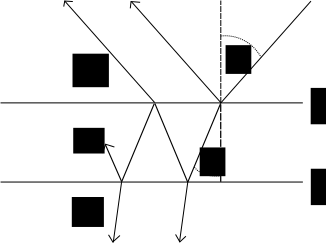
\includegraphics[width=10cm]{schema.png}
\caption{Schéma aparatury, K -- vysokofrekvenční zdroj mikrovln, VN -- zdroj vysokého napětí, M -- pentodový spínač, GM -- generátor pravoúhlých pulsů, V -- vlnoměr}
\label{schema}
\end{center}
\end{figure}

\section{Měření}
Měření bylo prováděno pro čtyři hodnoty tlaků: 50\,Pa, 100\,Pa, 200\,Pa a 500\,Pa. Naměřené hodnoty jsou v tabulkách \ref{p500},\ref{p200},\ref{p100},\ref{p50} a obrázku \ref{koncentrace}, závislost $1/n_\mathrm{e} = f(t)$ je na obrázku \ref{1n} a závislost $\mathrm{ln}\, n_\mathrm{e} = f(t)$ na obrázku \ref{lnn}.
Data byly nafitovány a byly určeny koeficienty $D$ a $\alpha$ pro různé tlaky. Pro tlaky kde daná závislost nebyla lineární na celém rozsahu hodnot byla fitována jen lineární část. Výsledky jsou v tabulce \ref{vysledky}.  

\begin{table}[htbp]
\begin{center}
\begin{tabular}{|c|c|c|c|c|}
\hline
$f'$[MHz] & $t[\mathrm{\mu s}]$ & $n_\mathrm{e}[10^{15}\mathrm{m}^{-3}]$ & $\frac{1}{n_\mathrm{e}} [10^{-16} \mathrm{m}^3]$ & ln $n_\mathrm{e}$ \\ \hline
2732,57 & 1640 & 0,507 & 19,71 & 33,86 \\ \hline
2733,10 & 1160 & 0,812 & 12,32 & 34,33 \\ \hline
2733,43 & 890 & 0,998 & 10,02 & 34,54 \\ \hline
2733,70 & 770 & 1,15 & 8,70 & 34,68 \\ \hline
2734,33 & 590 & 1,51 & 6,64 & 34,95 \\ \hline
2734,92 & 460 & 1,84 & 5,42 & 35,15 \\ \hline
2735,94 & 400 & 2,42 & 4,14 & 35,42 \\ \hline
2736,74 & 324 & 2,87 & 3,48 & 35,59 \\ \hline
2738,39 & 244 & 3,81 & 2,63 & 35,88 \\ \hline
2739,85 & 180 & 4,63 & 2,16 & 36,07 \\ \hline
2742,12 & 146 & 5,92 & 1,69 & 36,32 \\ \hline
2744,54 & 108 & 7,29 & 1,37 & 36,53 \\ \hline
2748,33 & 86 & 9,44 & 1,06 & 36,78 \\ \hline
2752,57 & 62 & 11,8 & 0,84 & 37,01 \\ \hline
\end{tabular}
\caption{$p$ = 500\,Pa, $f_0$ = 2731,669\,MHz}
\label{p500}
\end{center}
\end{table}

\begin{table}[htbp]
\begin{center}
\begin{tabular}{|c|c|c|c|c|}
\hline
$f'$[MHz] & $t[\mathrm{\mu s}]$ & $n_\mathrm{e}[10^{15}\mathrm{m}^{-3}]$ & $\frac{1}{n_\mathrm{e}} [10^{-16} \mathrm{m}^3]$ & ln $n_\mathrm{e}$ \\ \hline
2732,21 & 2100 & 0,372 & 26,88 & 33,55 \\ \hline
2732,63 & 1560 & 0,609 & 16,43 & 34,04 \\ \hline
2732,73 & 1160 & 0,668 & 14,97 & 34,14 \\ \hline
2733,28 & 860 & 0,981 & 10,20 & 34,52 \\ \hline
2733,64 & 760 & 1,18 & 8,45 & 34,71 \\ \hline
2733,94 & 610 & 1,35 & 7,39 & 34,84 \\ \hline
2734,51 & 470 & 1,67 & 5,97 & 35,05 \\ \hline
2735,01 & 296 & 1,96 & 5,10 & 35,21 \\ \hline
2735,91 & 232 & 2,47 & 4,05 & 35,44 \\ \hline
2736,74 & 144 & 2,94 & 3,40 & 35,62 \\ \hline
2739,76 & 82 & 4,65 & 2,15 & 36,08 \\ \hline
\end{tabular}
\caption{$p$ = 200\,Pa, $f_0$ = 2731,551\,MHz}
\label{p200}
\end{center}
\end{table}

\begin{table}[htbp]
\begin{center}
\begin{tabular}{|c|c|c|c|c|}
\hline
$f'$[MHz] & $t[\mathrm{\mu s}]$ & $n_\mathrm{e}[10^{14}\mathrm{m}^{-3}]$ & $\frac{1}{n_\mathrm{e}} [10^{-16} \mathrm{m}^3]$ & ln $n_\mathrm{e}$ \\ \hline
2731,97 & 1240 & 2,71 & 36,96 & 33,23 \\ \hline
2732,27 & 800 & 4,40 & 22,74 & 33,72 \\ \hline
2732,33 & 680 & 4,73 & 21,12 & 33,79 \\ \hline
2732,66 & 520 & 6,60 & 15,16 & 34,12 \\ \hline
2732,92 & 370 & 8,12 & 12,32 & 34,33 \\ \hline
2733,22 & 216 & 9,81 & 10,20 & 34,52 \\ \hline
2733,55 & 94 & 11,7 & 8,57 & 34,69 \\ \hline
2734,00 & 78 & 14,2 & 7,04 & 34,89 \\ \hline
\end{tabular}
\caption{$p$ = 100\,Pa, $f_0$ = 2731,491\,MHz}
\label{p100}
\end{center}
\end{table}

\begin{table}[htbp]
\begin{center}
\begin{tabular}{|c|c|c|c|c|}
\hline
$f'$[MHz] & $t[\mathrm{\mu s}]$ & $n_\mathrm{e}[10^{14}\mathrm{m}^{-3}]$ & $\frac{1}{n_\mathrm{e}} [10^{-16} \mathrm{m}^3]$ & ln $n_\mathrm{e}$ \\ \hline
2731,76 & 820 & 2,11 & 47,31 & 32,98 \\ \hline
2731,88 & 540 & 2,79 & 35,84 & 33,26 \\ \hline
2732,24 & 410 & 4,82 & 20,75 & 33,81 \\ \hline
2732,42 & 310 & 5,83 & 17,14 & 34,00 \\ \hline
2732,80 & 196 & 8,03 & 12,45 & 34,32 \\ \hline
2733,10 & 136 & 9,72 & 10,28 & 34,51 \\ \hline
2733,25 & 96 & 10,6 & 9,46 & 34,59 \\ \hline
2733,58 & 74 & 12,4 & 8,05 & 34,76 \\ \hline
2733,88 & 50 & 14,1 & 7,08 & 34,88 \\ \hline
\end{tabular}
\end{center}
\caption{$p$ = 50\,Pa, $f_0$ = 2731,386\,MHz}
\label{p50}
\end{table}

\begin{figure}[htbp]
\begin{center}
\includegraphics[width=13.5cm]{Graph1.pdf}
\caption{Vývoj elektronové koncentrace ve vyhasínajícím plazmatu v závislosti na čase pro různé tlaky}
\label{koncentrace}
\end{center}
\end{figure}

\begin{figure}[htbp]
\begin{center}
\includegraphics[width=13.5cm]{Graph2.pdf}
\caption{Závislost $\frac{1}{n_\mathrm{e}} = f(t)$ pro různé tlaky}
\label{1n}
\end{center}
\end{figure}

\begin{figure}[htbp]
\begin{center}
\includegraphics[width=13.5cm]{Graph3.pdf}
\caption{Závislost $\mathrm{ln}\, n_\mathrm{e} = f(t)$  pro různé tlaky}
\label{lnn}
\end{center}
\end{figure}

\begin{table}[htbp]
\begin{center}
\begin{tabular}{|c|c|c|c|c|c|}
\hline
$p$[Pa] & $D$ [10$^{-2}$m$^2$s$^{-1}$] & $\sigma_D$[10$^{-4}$m$^2$s$^{-1}$] & $\alpha$[10$^{-12}$m$^2$s$^{-1}$] & $\sigma_\alpha$[10$^{-14}$m$^2$s$^{-1}$] & $n_{\mathrm{eq}}$[10$^{14}$m$^{-3}$] \\ \hline
500 & 1,485 & 9,9 & 1,154 & 2,522 & 9,185 \\ \hline
200 & 1,284 & 9,7 & 1,140 & 6,087 & 8,046 \\ \hline
100 & 1,936 & 11 & 1,673 & 14,59 & 8,262 \\ \hline
50 & 3,544 & 26 & 3,763 & 8,686 & 6,723 \\ \hline
\end{tabular}
\caption{Výsledky, $n_\mathrm{eq}$ je hodnota koncentrace při které jsou difuzní i rekombinační ztráty stejné.}
\label{vysledky}
\end{center}
\end{table}

\begin{figure}[htbp]
\begin{center}
\includegraphics[width=13.5cm]{Graph4.pdf}
\caption{Výsledky}
\label{vysledkyimg}
\end{center}
\end{figure}

\section{Závěr}
Měření bylo úspěšné, podařilo se naměřit vývoj elektronové koncentrace ve vyhasínajícím plazmatu v závislosti na čase pro různé tlaky. Analýzou grafů $\mathrm{ln}\,n_\mathrm{e} = f(t)$ a $1/n_\mathrm{e} = f(t)$ se potvrdilo, že při vyšších koncentracích převládá rekombinace, při nižších difuze. Pro všechny čtyři naměřené tlaky nicméně můžeme v grafech vidět že výsledná závislost je kombinaci obou jevů, pro tlaky 500\,Pa a 100\,Pa převládá rekombinace, pro 100\,Pa a 50\,Pa převládá difuze. Fitováním výše uvedených závislostí byly spočítány rekombinační a difuzní koeficienty. Ukázalo se, že rekombinační i difuzní koeficient rostou s klesajícím tlakem. To si vysvětluji menší koncentrací neutrálů, přičemž srážky s nimi brzdí difuzi.
\newpage

\section{Dodatek}
Předchozí vyhodnocení předpokládalo výskyt pouze jednoho typu úbytku nabitých částic, buď rekombinace nebo difuze. Ve skutečnosti ale v plazmatu probíhají vždy oba procesy. Rovnice pro změnu koncentrace v případě že započítáme oba dva procesy vypadá následovně

\begin{equation}
-\frac{\mathrm{d}n(t)}{\mathrm{d}t} = \alpha n^2(t) + \frac{D}{\Lambda^2}n(t) \mathrm{.}
\end{equation}
Řešení má tvar
\begin{equation}
n(t)=  -\frac{ \frac{D}{\Lambda^2} }{ \alpha - C \frac{D}{\Lambda^2} \mathrm{exp}(\frac{D}{\Lambda^2} t) } \mathrm{.}
\end{equation}
Počáteční podmínka je $n(0) = n_0$, to vede na rovnici
\begin{equation}
n(t)=  -\frac{ \frac{D}{\Lambda^2} }{ \alpha - (\frac{\alpha}{\frac{D}{\Lambda^2}} + \frac{1}{n_0})\, \frac{D}{\Lambda^2} \,\mathrm{exp}(\frac{D}{\Lambda^2} t ) } \mathrm{.}
\end{equation}

Nyní můžeme přistoupit k fitování naměřených závislostí odvozeným novým vzorcem.

\begin{figure}[htbp]
\begin{center}
\includegraphics[width=13cm]{fit500pa.pdf}
\caption{Fit časového vývoje elektronové koncentrace pro $p$=500\,Pa}
\label{fit500}
\end{center}
\end{figure}

\begin{figure}[htbp]
\begin{center}
\includegraphics[width=13cm]{fit200pa.pdf}
\caption{Fit časového vývoje elektronové koncentrace pro $p$=200\,Pa, fit 1 má oproti fitu 2 o více než jeden řád lepší reziduální sumu čtverců, ale difuzní koeficient vychází záporně, u fitu 2 jsem proto fitování difuzního koeficientu omezil pouze na kladné hodnoty.}
\label{fit200}
\end{center}
\end{figure}

\begin{figure}[htbp]
\begin{center}
\includegraphics[width=13cm]{fit100Pa.pdf}
\caption{Fit časového vývoje elektronové koncentrace pro $p$=100\,Pa}
\label{fit100}
\end{center}
\end{figure}

\begin{figure}[htbp]
\begin{center}
\includegraphics[width=13cm]{fit50Pa.pdf}
\caption{Fit časového vývoje elektronové koncentrace pro $p$=50\,Pa}
\label{fit50}
\end{center}
\end{figure}

\begin{figure}[htbp]
\begin{center}
\includegraphics[width=12cm]{difuzefinal.pdf}
\caption{Porovnání difuzních koeficientů získaných původním (zjednodušeným) postupem a fitováním přesného řešení}
\label{difuzefinal}
\end{center}
\end{figure}

\begin{figure}[htbp]
\begin{center}
\includegraphics[width=12cm]{rekombfinal.pdf}
\caption{Porovnání rekombinačních koeficientů získaných původním (zjednodušeným) postupem a fitováním přesného řešení}
\label{rekombfinal}
\end{center}
\end{figure}

\begin{table}[htbp]
\begin{center}
\begin{tabular}{|c|c|c|c|c|c|c|}
\hline
P [Pa] & $\alpha$[10$^{-12}$m$^2$s$^{-1}$] & $\sigma_\alpha$[10$^{-13}$m$^2$s$^{-1}$] & $D$ [10$^{-3}$m$^2$s$^{-1}$] & $\sigma_D$[10$^{-3}$m$^2$s$^{-1}$] & $n_{\mathrm{e}}$[10$^{15}$m$^{-3}$] & $\sigma_{n_{\mathrm{e}}}$[10$^{15}$m$^{-3}$] \\ \hline
500 & 1,025 & 0,505 & 1,567& 2,946 & 49,49 & 7,822  \\ \hline
200 & 0,501 & 6,922 & 8,681 & 13,89 & 3,831 & 2,385  \\ \hline
100 & 1,100 & 8,772 & 9,686 & 9,504 & 1,575 & 0,132  \\ \hline
50 & 2,753 & 8,377 & 14,69 & 8,573 & 1,814 & 0,121 \\ \hline
\end{tabular}
\end{center}
\caption{}
\label{}
\end{table}

\newpage

\section{Závěr dodatku}
Ukázalo se že původní postup, tedy předpoklad vždy pouze jednoho jevu, byl velmi nepřesný. Při měřených hodnotách elektronové koncentrace se vyskytují současně rekombinace i difuze. Toto se projevilo tím, že původní hodnoty difuzního i rekombinačního koeficientu jsou výrazně vyšší než hodnoty získané v dodatku. To je proto, že původní model počítal s přítomností buď pouze difuze a nebo pouze rekombinace a tím pádem současná přítomnost druhého jevu způsobila vyšší hodnotu koeficientů. Nevýhodou fitování přesným analytickým řešením je jeho značná složitost která má na svědomí větší chyby. Také bylo potřeba velmi opatrně volit počáteční veličiny pro fit, jinak model vůbec nekonvergoval (zde se velmi hodily předchozí výsledky), a navíc při neopatrném fitování můžeme jednoduše dostat výsledky které nedávají fyzikální smysl (jako například na obrázku \ref{fit200}). 



\end{document}
